% !TeX program = xelatex
\documentclass[
  convert={density=500, size=600, outext=.png}, 
  border=2pt
]{standalone}

\usepackage{fontspec}
\defaultfontfeatures{Ligatures={NoCommon,%
			NoDiscretionary,%
			NoHistoric,%
			NoRequired,%
			NoContextual}}
\setsansfont{Carlito}[%
	SmallCapsFeatures={Letters=SmallCaps},%
	SmallCapsFont={Roboto},%
	ItalicFeatures={SmallCapsFont=Roboto-Italic},%
	BoldFeatures={SmallCapsFont=Roboto-Bold},%
	BoldItalicFeatures={SmallCapsFont=Roboto-BoldItalic}%
]

\usepackage{tikz}
\usepackage{tikz-cd}
\usetikzlibrary{%
	calc,%
	arrows.meta,%
	arrows,%
	automata,%
	overlay-beamer-styles,%
	snakes,%
	shapes.arrows,%
	shapes.geometric,%
	shapes.symbols,%
	fit,%
	positioning,%
	decorations.pathreplacing,%
	backgrounds,%
}
\tikzset{
	>=Triangle,%
	nodes={align=center},%
	comp/.style={%
			draw,%
			rectangle,%
			very thick,%
			rounded corners,%
			minimum width=2.5cm,%
			minimum height=1cm,%
			fill=white},%
	input/.style={draw,%
			rectangle,%
			thick,%
			minimum width=2.5cm,%
			minimum height=1cm,%
			fill=white},%
	classnode/.style={%
			fill=cgreenlight,%
			rectangle,%
			draw,%
			inner xsep=0},%
	interfacenode/.style={%
			fill=corangelight,%
			rectangle,%
			draw,%
			inner xsep=0},%
	abstractclassnode/.style={%
			fill=cbluelight,%
			rectangle,%
			draw,%
			inner xsep=0},%
	inlinenode/.style={%
			inner xsep=.5cm,%
			minimum height=.6cm},%
}

\definecolor{reddy}{RGB}{172, 0, 51}
\definecolor{dkred}{rgb}{.6, 0, 0}
\definecolor{dkgreen}{rgb}{0, .5, 0}
\definecolor{dkblue}{rgb}{0, 0, .5}
\definecolor{cred}{RGB}{219, 68, 55}
\definecolor{credlight}{RGB}{250, 227, 225}
\definecolor{cgreen}{RGB}{3, 148, 77}
\definecolor{cgreenlight}{RGB}{209, 251, 230}
\definecolor{cblue}{RGB}{2, 119, 189}
\definecolor{cbluelight}{RGB}{208, 237, 254}
\definecolor{corange}{RGB}{173, 128, 2}
\definecolor{corangelight}{RGB}{253, 219, 123}
\newcommand{\cblue}[1]{\textcolor{cblue}{#1}}
\newcommand{\bfcblue}[1]{\textcolor{cblue}{\textbf{#1}}}
\newcommand{\cred}[1]{\textcolor{cred}{#1}}
\newcommand{\bfcred}[1]{\textcolor{cred}{\textbf{#1}}}
\newcommand{\cgreen}[1]{\textcolor{cgreen}{#1}}
\newcommand{\bfcgreen}[1]{\textcolor{cgreen}{\textbf{#1}}}
\newcommand{\corange}[1]{\textcolor{corange}{#1}}
\newcommand{\bfcorange}[1]{\textcolor{corange}{\textbf{#1}}}
\newcommand{\interfacename}[1]{\underline{\textbf{\textit{#1}}}}
\newcommand{\absclassname}[1]{\textbf{\textit{#1}}}
\newcommand{\classname}[1]{\textbf{#1}}

\usepackage{amsmath}
\usepackage{amsfonts}
\usepackage{amssymb}

\usepackage{silence}
\WarningsOff*


\begin{document}
\sffamily

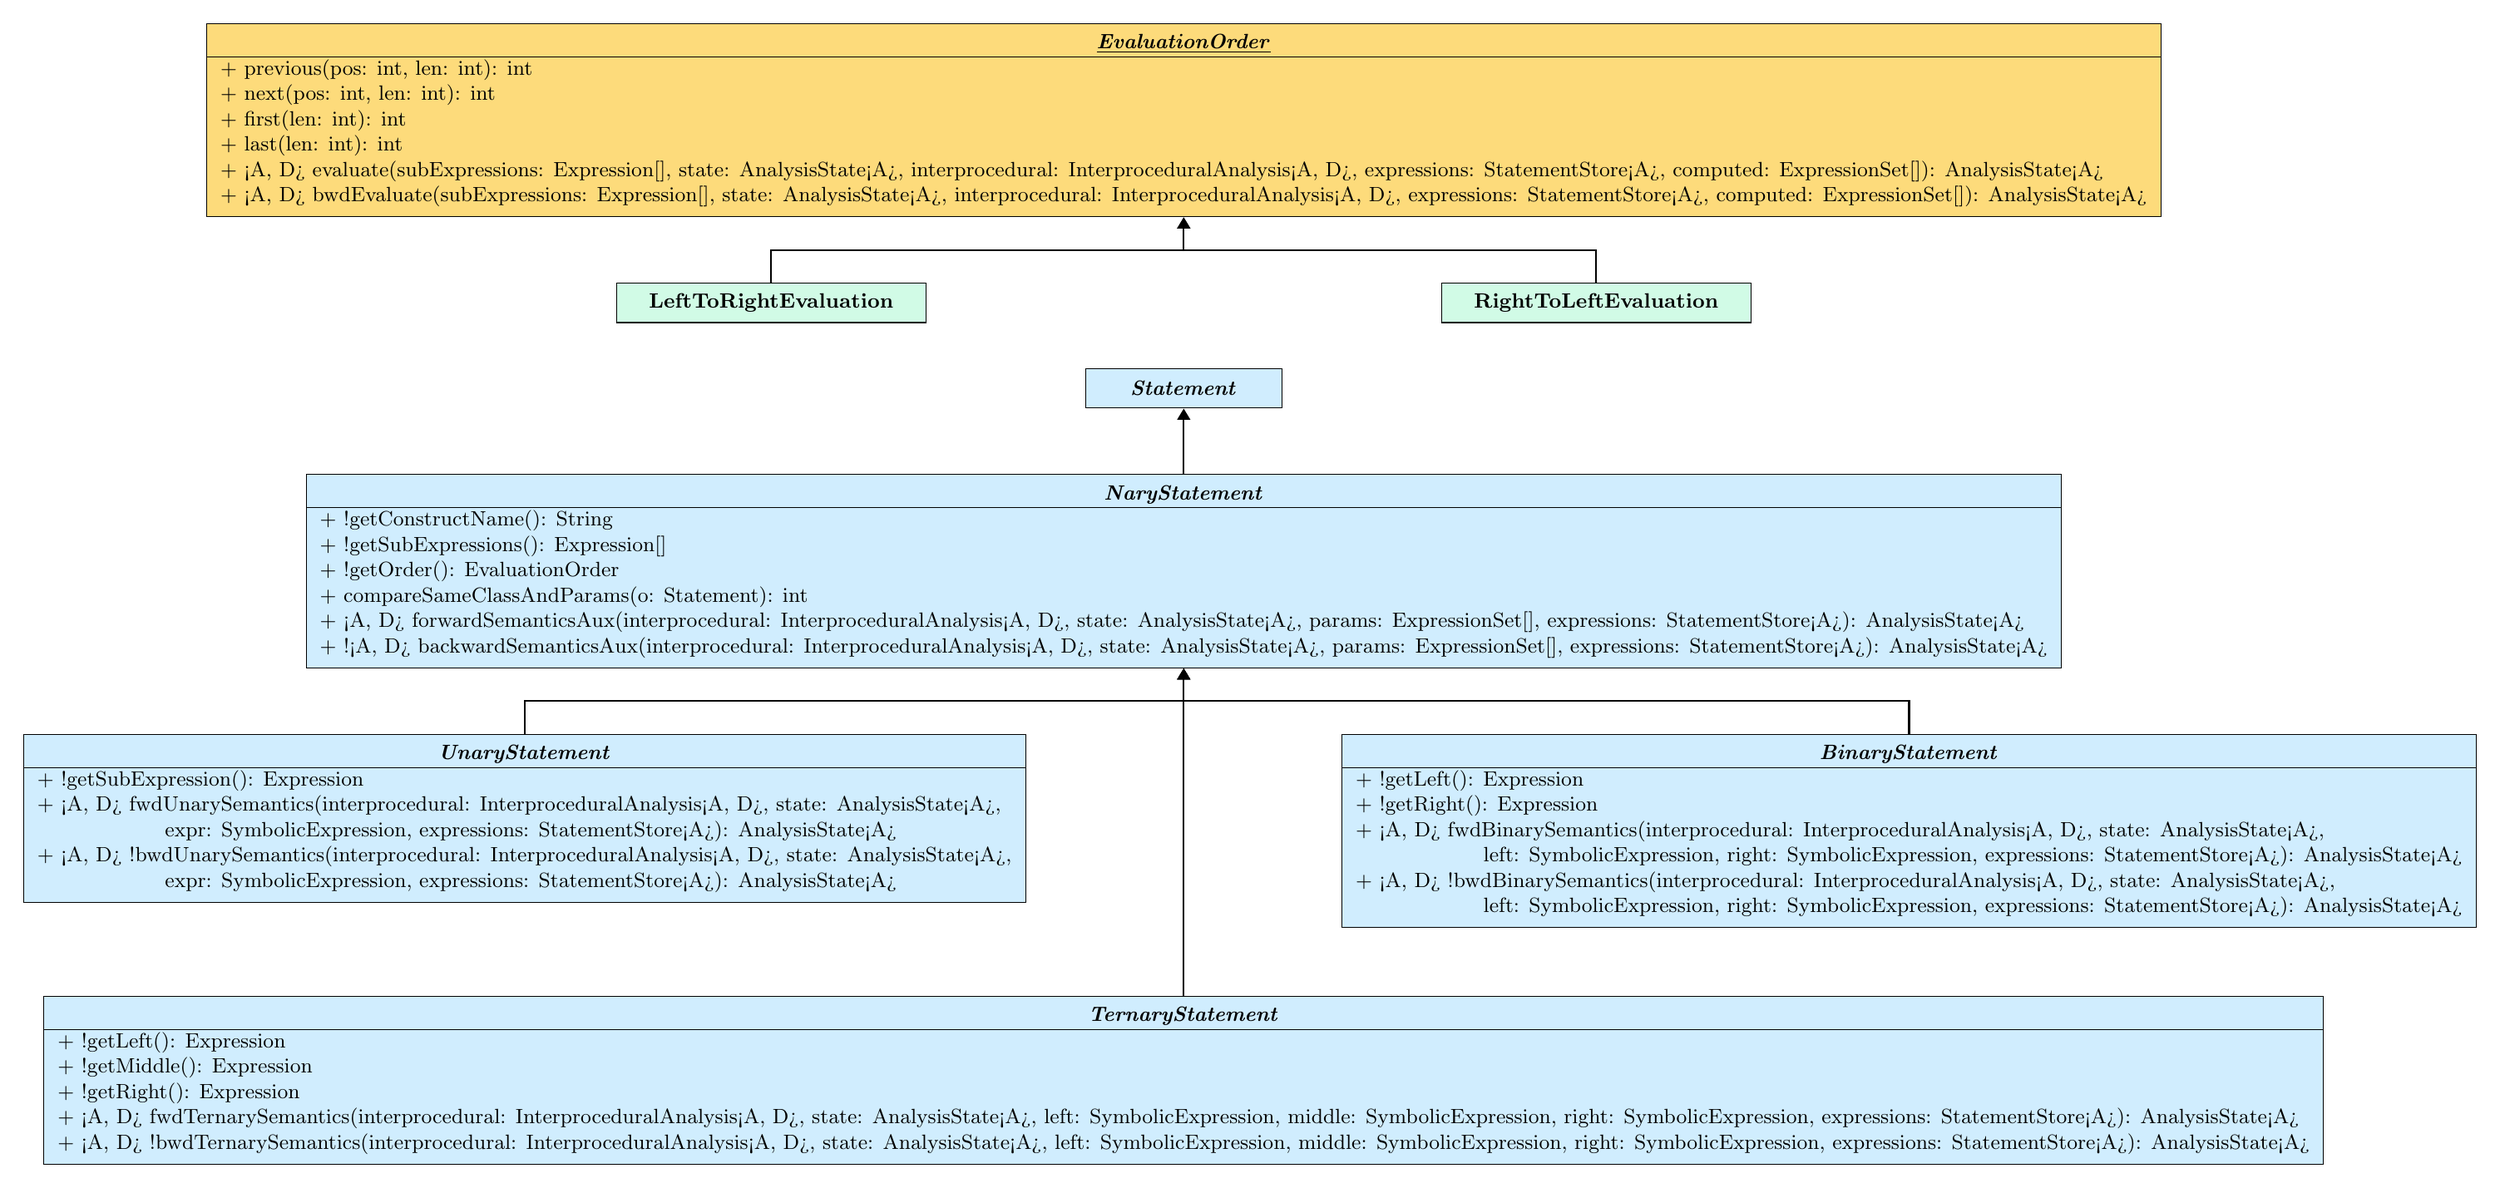
\begin{tikzpicture}[nodes={font={\small}, minimum width=3cm}]%
	\node[interfacenode] (eval) {\begin{tabular}{l}
			\multicolumn{1}{c}{\interfacename{EvaluationOrder}}                                                                                                                                                      \\
			\hline
			+ previous(pos: int, len: int): int                                                                                                                                                                      \\
			+ next(pos: int, len: int): int                                                                                                                                                                          \\
			+ first(len: int): int                                                                                                                                                                                   \\
			+ last(len: int): int                                                                                                                                                                                    \\
			+ <A, D> evaluate(subExpressions: Expression[], state: AnalysisState<A>, interprocedural: InterproceduralAnalysis<A, D>, expressions: StatementStore<A>, computed: ExpressionSet[]): AnalysisState<A>    \\
			+ <A, D> bwdEvaluate(subExpressions: Expression[], state: AnalysisState<A>, interprocedural: InterproceduralAnalysis<A, D>, expressions: StatementStore<A>, computed: ExpressionSet[]): AnalysisState<A> \\
		\end{tabular}};

	\node[classnode, inlinenode] (leval) [below left=1cm and -11cm of eval] {\classname{LeftToRightEvaluation}};
	\node[classnode, inlinenode] (reval) [below right=1cm and -11cm of eval] {\classname{RightToLeftEvaluation}};

	\node[abstractclassnode, inlinenode] (st) [below=of $(leval)!0.5!(reval)$] {\absclassname{Statement}};

	\node[abstractclassnode] (nst) [below=of st] {\begin{tabular}{l}
			\multicolumn{1}{c}{\absclassname{NaryStatement}}                                                                                                                                  \\
			\hline
			+ !getConstructName(): String                                                                                                                                                     \\
			+ !getSubExpressions(): Expression[]                                                                                                                                              \\
			+ !getOrder(): EvaluationOrder                                                                                                                                                    \\
			+ compareSameClassAndParams(o: Statement): int                                                                                                                                    \\
			+ <A, D> forwardSemanticsAux(interprocedural: InterproceduralAnalysis<A, D>, state: AnalysisState<A>,  params: ExpressionSet[], expressions: StatementStore<A>): AnalysisState<A> \\
			+ !<A, D> backwardSemanticsAux(interprocedural: InterproceduralAnalysis<A, D>, state: AnalysisState<A>, params: ExpressionSet[], expressions: StatementStore<A>): AnalysisState<A> \\
		\end{tabular}};

	\node[abstractclassnode] (bst) [below right=1cm and -11cm of nst] {\begin{tabular}{l}
			\multicolumn{1}{c}{\absclassname{BinaryStatement}}                                                                           \\
			\hline
			+ !getLeft(): Expression                                                                                                     \\
			+ !getRight(): Expression                                                                                                    \\
			+ <A, D> fwdBinarySemantics(interprocedural: InterproceduralAnalysis<A, D>, state: AnalysisState<A>,                         \\
			$\qquad\qquad\qquad$left: SymbolicExpression, right: SymbolicExpression, expressions:  StatementStore<A>):  AnalysisState<A> \\
			+ <A, D> !bwdBinarySemantics(interprocedural: InterproceduralAnalysis<A, D>, state: AnalysisState<A>,                        \\
			$\qquad\qquad\qquad$left: SymbolicExpression, right: SymbolicExpression, expressions: StatementStore<A>): AnalysisState<A>   \\
		\end{tabular}};

	\node[abstractclassnode] (ust) [below left=1cm and -11cm of nst] {\begin{tabular}{l}
			\multicolumn{1}{c}{\absclassname{UnaryStatement}}                                                    \\
			\hline
			+ !getSubExpression(): Expression                                                                    \\
			+ <A, D> fwdUnarySemantics(interprocedural: InterproceduralAnalysis<A, D>, state: AnalysisState<A>,  \\
			$\qquad\qquad\qquad$expr: SymbolicExpression, expressions:  StatementStore<A>):  AnalysisState<A>    \\
			+ <A, D> !bwdUnarySemantics(interprocedural: InterproceduralAnalysis<A, D>, state: AnalysisState<A>, \\
			$\qquad\qquad\qquad$expr: SymbolicExpression, expressions: StatementStore<A>): AnalysisState<A>      \\
		\end{tabular}};

	\node[abstractclassnode] (tst) [below=5cm of nst] {\begin{tabular}{l}
			\multicolumn{1}{c}{\absclassname{TernaryStatement}}                                                                                                                                                                                        \\
			\hline
			+ !getLeft(): Expression                                                                                                                                                                                                                   \\
			+ !getMiddle(): Expression                                                                                                                                                                                                                 \\
			+ !getRight(): Expression                                                                                                                                                                                                                  \\
			+ <A, D> fwdTernarySemantics(interprocedural: InterproceduralAnalysis<A, D>, state: AnalysisState<A>, left: SymbolicExpression, middle: SymbolicExpression, right: SymbolicExpression, expressions:  StatementStore<A>):  AnalysisState<A> \\
			+ <A, D> !bwdTernarySemantics(interprocedural: InterproceduralAnalysis<A, D>, state: AnalysisState<A>, left: SymbolicExpression, middle: SymbolicExpression, right: SymbolicExpression, expressions: StatementStore<A>): AnalysisState<A>  \\
		\end{tabular}};

	\draw[->, thick] (nst) to (st);
	\draw[->, thick] (ust) |- ($(nst.south)+(0,-0.5)$) to (nst);
	\draw[->, thick] (bst) |- ($(nst.south)+(0,-0.5)$) to (nst);
	\draw[->, thick] (tst) to (nst);
	\draw[->, thick] (leval) |- ($(eval.south)+(0,-0.5)$) to (eval);
	\draw[->, thick] (reval) |- ($(eval.south)+(0,-0.5)$) to (eval);
\end{tikzpicture}

\end{document}
